\documentclass[12pt]{article}
\usepackage{graphicx}
\usepackage{amsmath}
\begin{center}
\textbf{Varad Madan Karmarkar}
\end{center}
\hline
\label{sec:VaradMadanKarmarkar}
\begin{document}
\begin{flushleft}
83/B/2\hspace{2.8in} Contact:9503502432\\ 
Gandharva Palace\hspace{1in} Email Id:varadkarmarkar.v.k@gmail.com\\ 
Kasbekar Park,\\ 
Kolhapur-416003,\\ 
Maharashtra.
\vspace{-4ex}
\begin{figure}[h]
	\begin{flushright}
		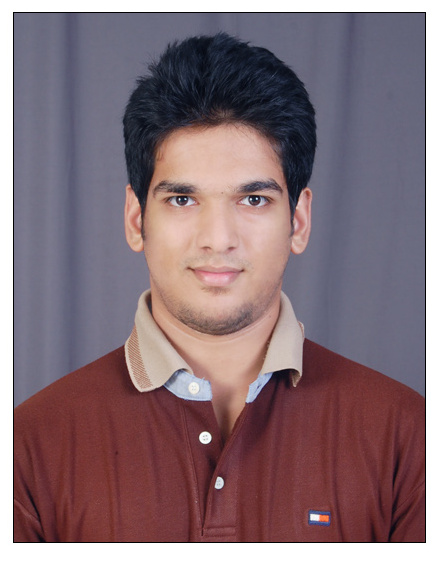
\includegraphics[width=0.2\linewidth,angle=+0]{F:/vkphoto.jpg}
	\label{fig:vkphoto}
	\end{flushright}
\end{figure}
\vspace{-4ex}
\begin{flushleft}
\textbf{OBJECTIVE}: To involve myself in a challenging and healthy work environment offering scope for growth & development and an opportunity to apply my knowledge to effectively contribute towards the achievement of the organizational objective. }
\end{flushleft}
\begin{flushleft}
\caption{\textbf{EDUCATION:}}\vspace{2ex}
\begin{tabular}{|l|c|c|c|c|r|}  \hline
Degree & College/School & University & Passing Year &  Percentage\\ \hline
B.Tech & Walchand COE, & Shivaji & 2017 & 9.1\\ 
Electrical & Sangli & University & & (CPI) \\ \hline
\end{tabular}
\end{flushleft}
\begin{flushleft}
\textbf{PROJECTS:}
\end{flushleft}
\begin{enumerate}
\item Self-regulatory dual dc voltage bus bar system in vehicles using PID control under the guidance of Dr. D R Patil
\item  Automatic lighting control using instrumentation amplifier.
\item Image processing based autonomous robot using camera for eYRC+. 
\end{enumerate}
\begin{flushleft}
\textbf{TRAINING AND INTERNSHIP :}
\begin{itemize}
\item Industrial Training at �Traction Machine Workshop, Nashik�, from 16th July 2015
to 25th July 2015.
\item Industrial Training at �Power Engineers (Transformer manufacturing), Kolhapur�, from 26th May 2015 to 12th June 2015.
\end{itemize}
\end{flushleft}
\begin{flushleft}
\textbf{RESEARCH AND PUBLICATIONS:}\\
1.
\end{flushleft}
\begin{flushleft}
\textbf{TECHNICAL SKILLS : }
\begin{itemize}
\item \textbf{Softwares known:} Microsoft Office 2010, Turbo C, Python(novice), Matlab 2015, Proteus, Keil UVision, Zelio-Soft 2 (PLC), Ignition SCADA (novice), Arduino.
\item PCB designing using Proteus.
\item Power Electronics and Arduino, 8051, Raspberry-Pi micro-controllers.
\end{itemize}
\end{flushleft}
\begin{flushleft}
\textbf{SOFT SKILLS:}
\begin{enumerate}
\item Responsible Nature.
\item Multitasking Skills.
\item Team Player. 
\end{enumerate}
\begin{flushleft}
\textbf{EXTRA CURRICULAR ACTIVITIES :}
\begin{itemize}
\item Member Of Electrical Engineering Students Association (EESA).
\item Playing Badminton
\end{itemize}
\end{flushleft}
\textbf{CO-CURRICULAR ACTIVITIES : }
\begin{enumerate}
\item \textbf{Winner} in the event Courier Services in E-Yantra+ 2016, a national level robotics competition by IIT-Bombay.
\item \textbf{Winner} in the event $\mu$-ERA (8085 PROGRAMMING) in ELECTROVERT 2014, a state level technical symposium by ELESA.
\item \textbf{Workshops Attended}\\ 1. PLC and SCADA held by ETA (Educate to Automate).\\
2.Solar and smart energy systems held by Roboversity.
\end{enumerate}
\textbf{PERSONAL DETAILS:}\\
\vspace{2ex}
Father's Name : Madan Ramkrishna Karmarkar\\
Mother's Name : Suvarna Madan Karmarkar\\
Birth date : 31st May, 1996\\
Gender : Male\\
Nationality : Indian\\
Languages known : English, Marathi, Hindi\\
\vspace{5ex}
\textbf{Declaration:}\\The above information is true to the best of my knowledge and belief.\\
\vspace{5ex}
\textbf{Date:} 21st May 2016
\end{flushleft}
\end {document}
